
\subsection{Diseño}


\begin{itemize}

  \item \textbf{Diagrama Entidad - Relación:}

En la figura \ref{fig:er_ubikate}, se observa el diagrama Entidad - Relación de la aplicación.


\begin{figure}[H]
  \begin{center}
    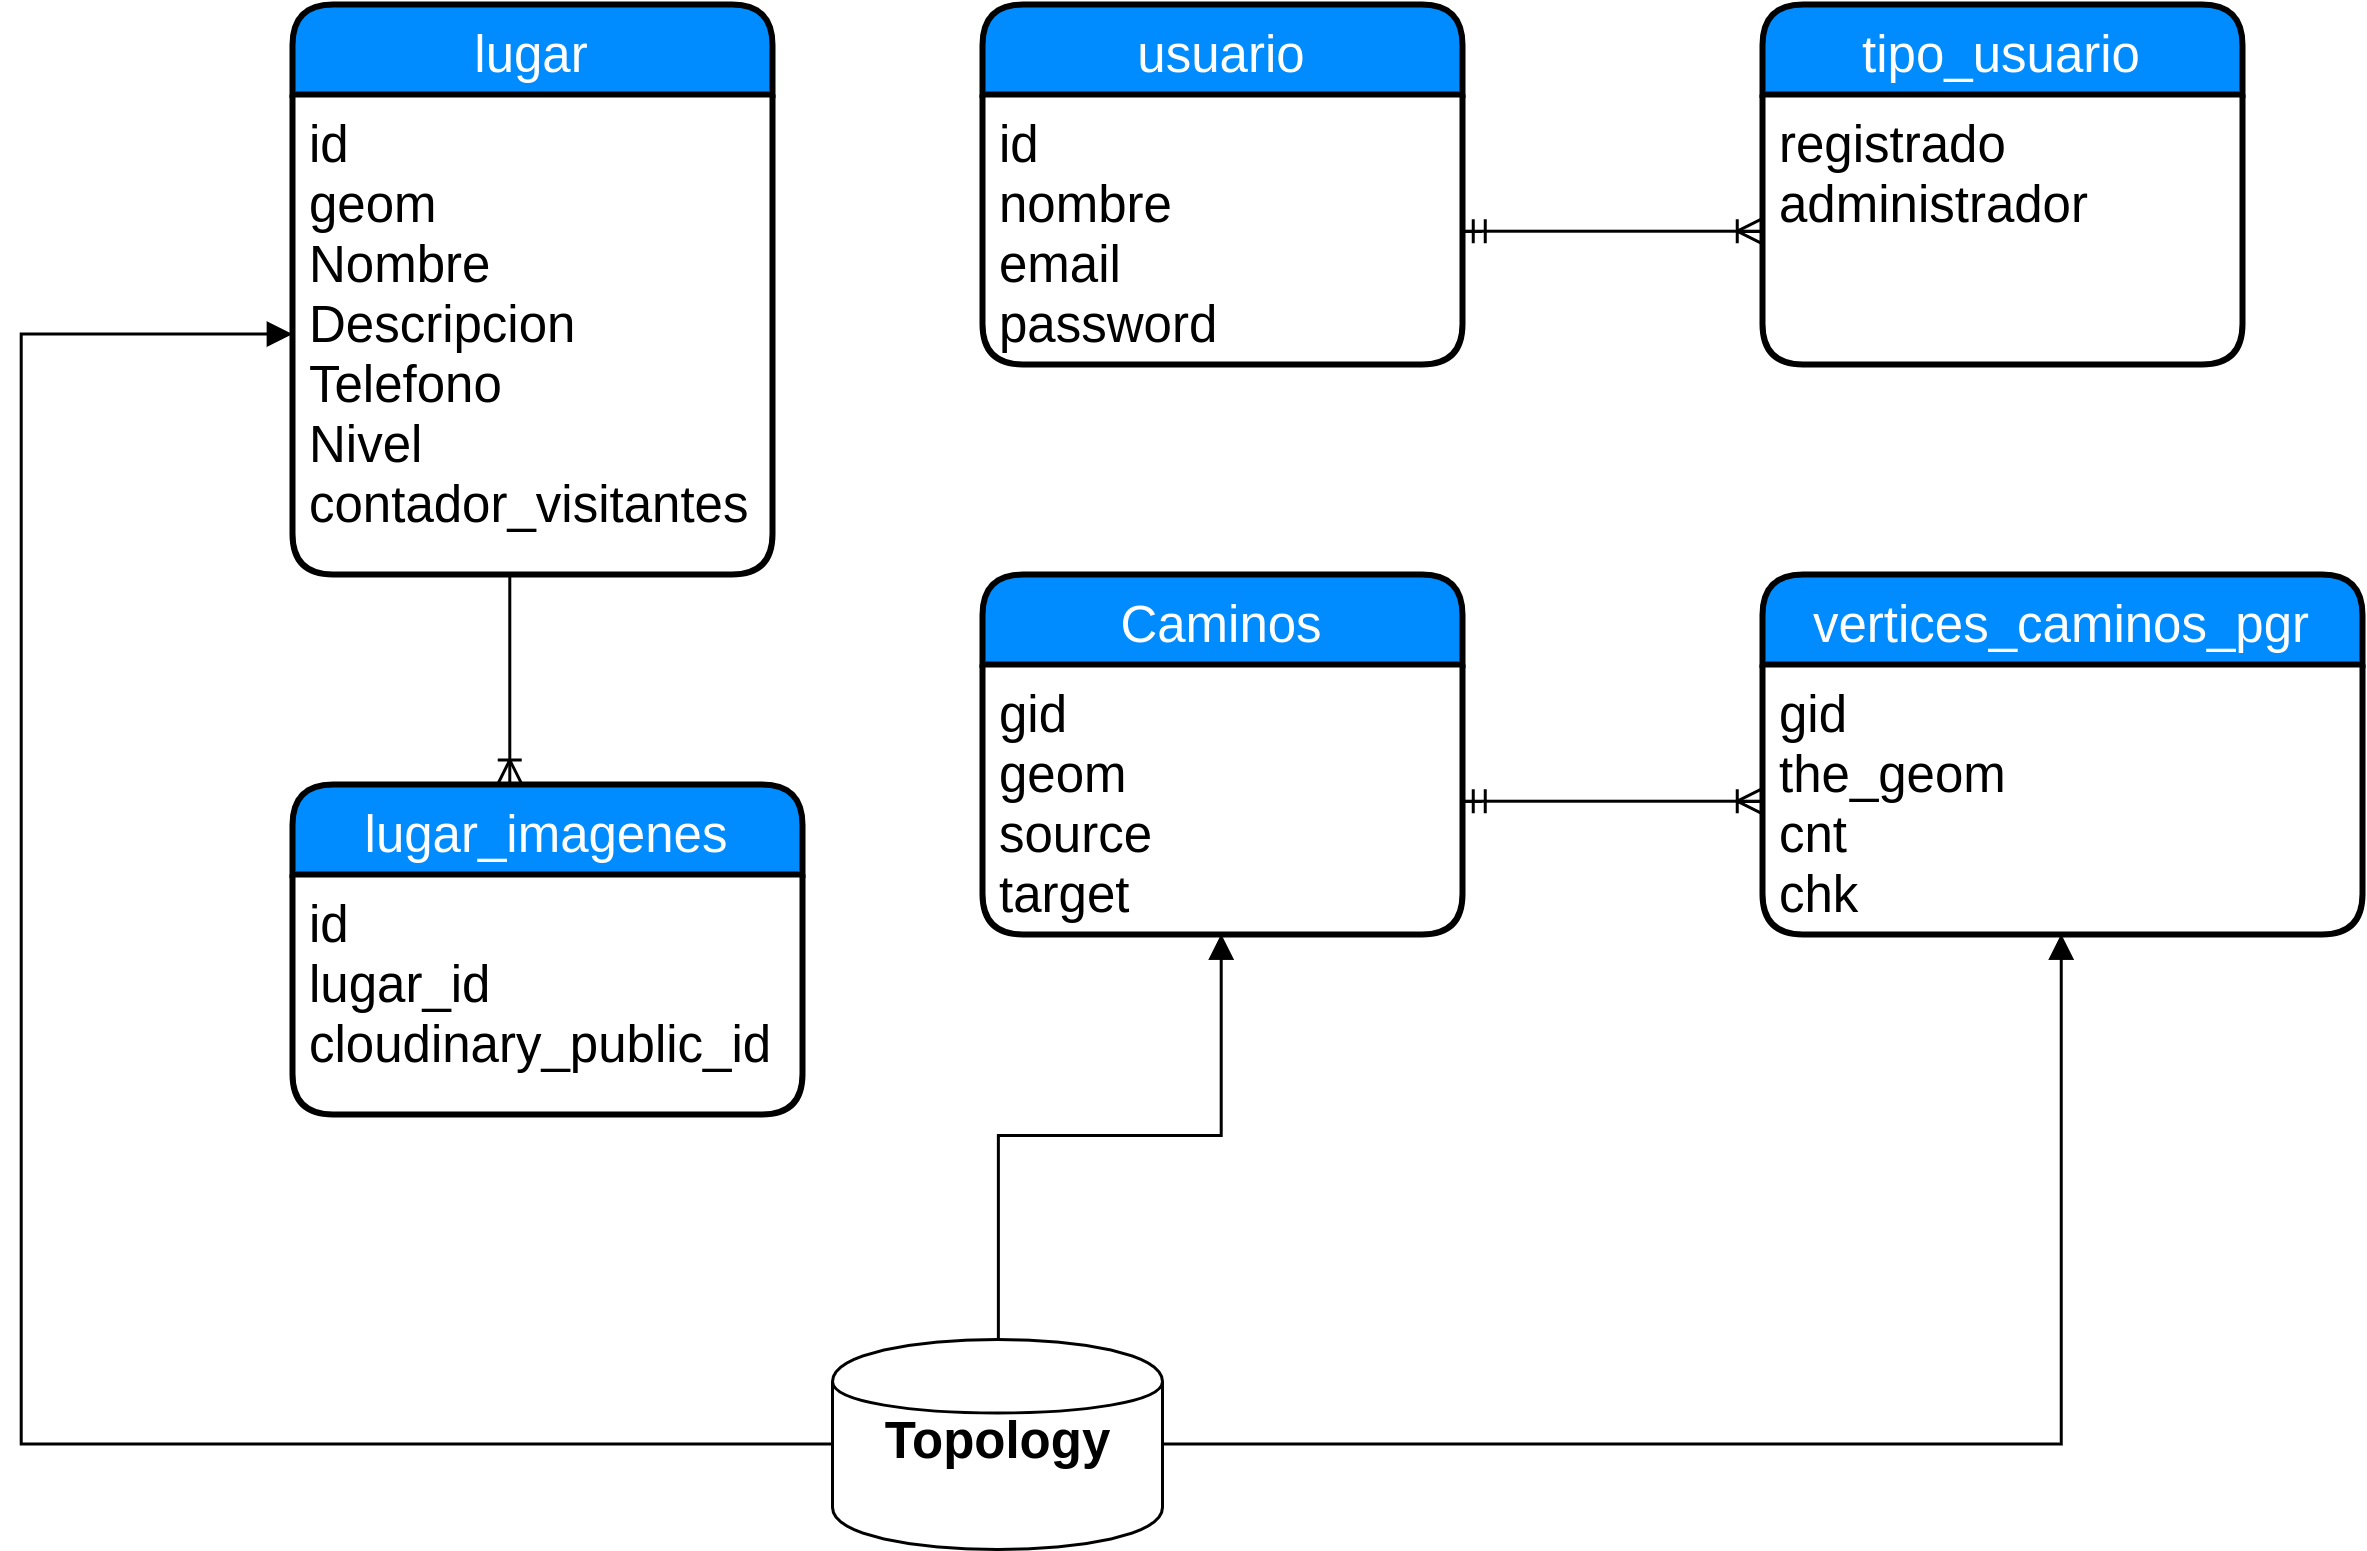
\includegraphics[width=0.8\textwidth]{diagramas/er_ubikate}
  \end{center}
  \caption{Diagrama ER: Ubikate UMSS}
  \label{fig:er_ubikate}
  \caption*{Fuente: Elaboración propia}
\end{figure}


\item \textbf{Diagrama de Secuencia:}

En la figura \ref{fig:sequence_registrar_usuario}, se observa el diagrama de secuencia correspondiente al registro de un usuario.

\begin{figure}[H]
  \begin{center}
    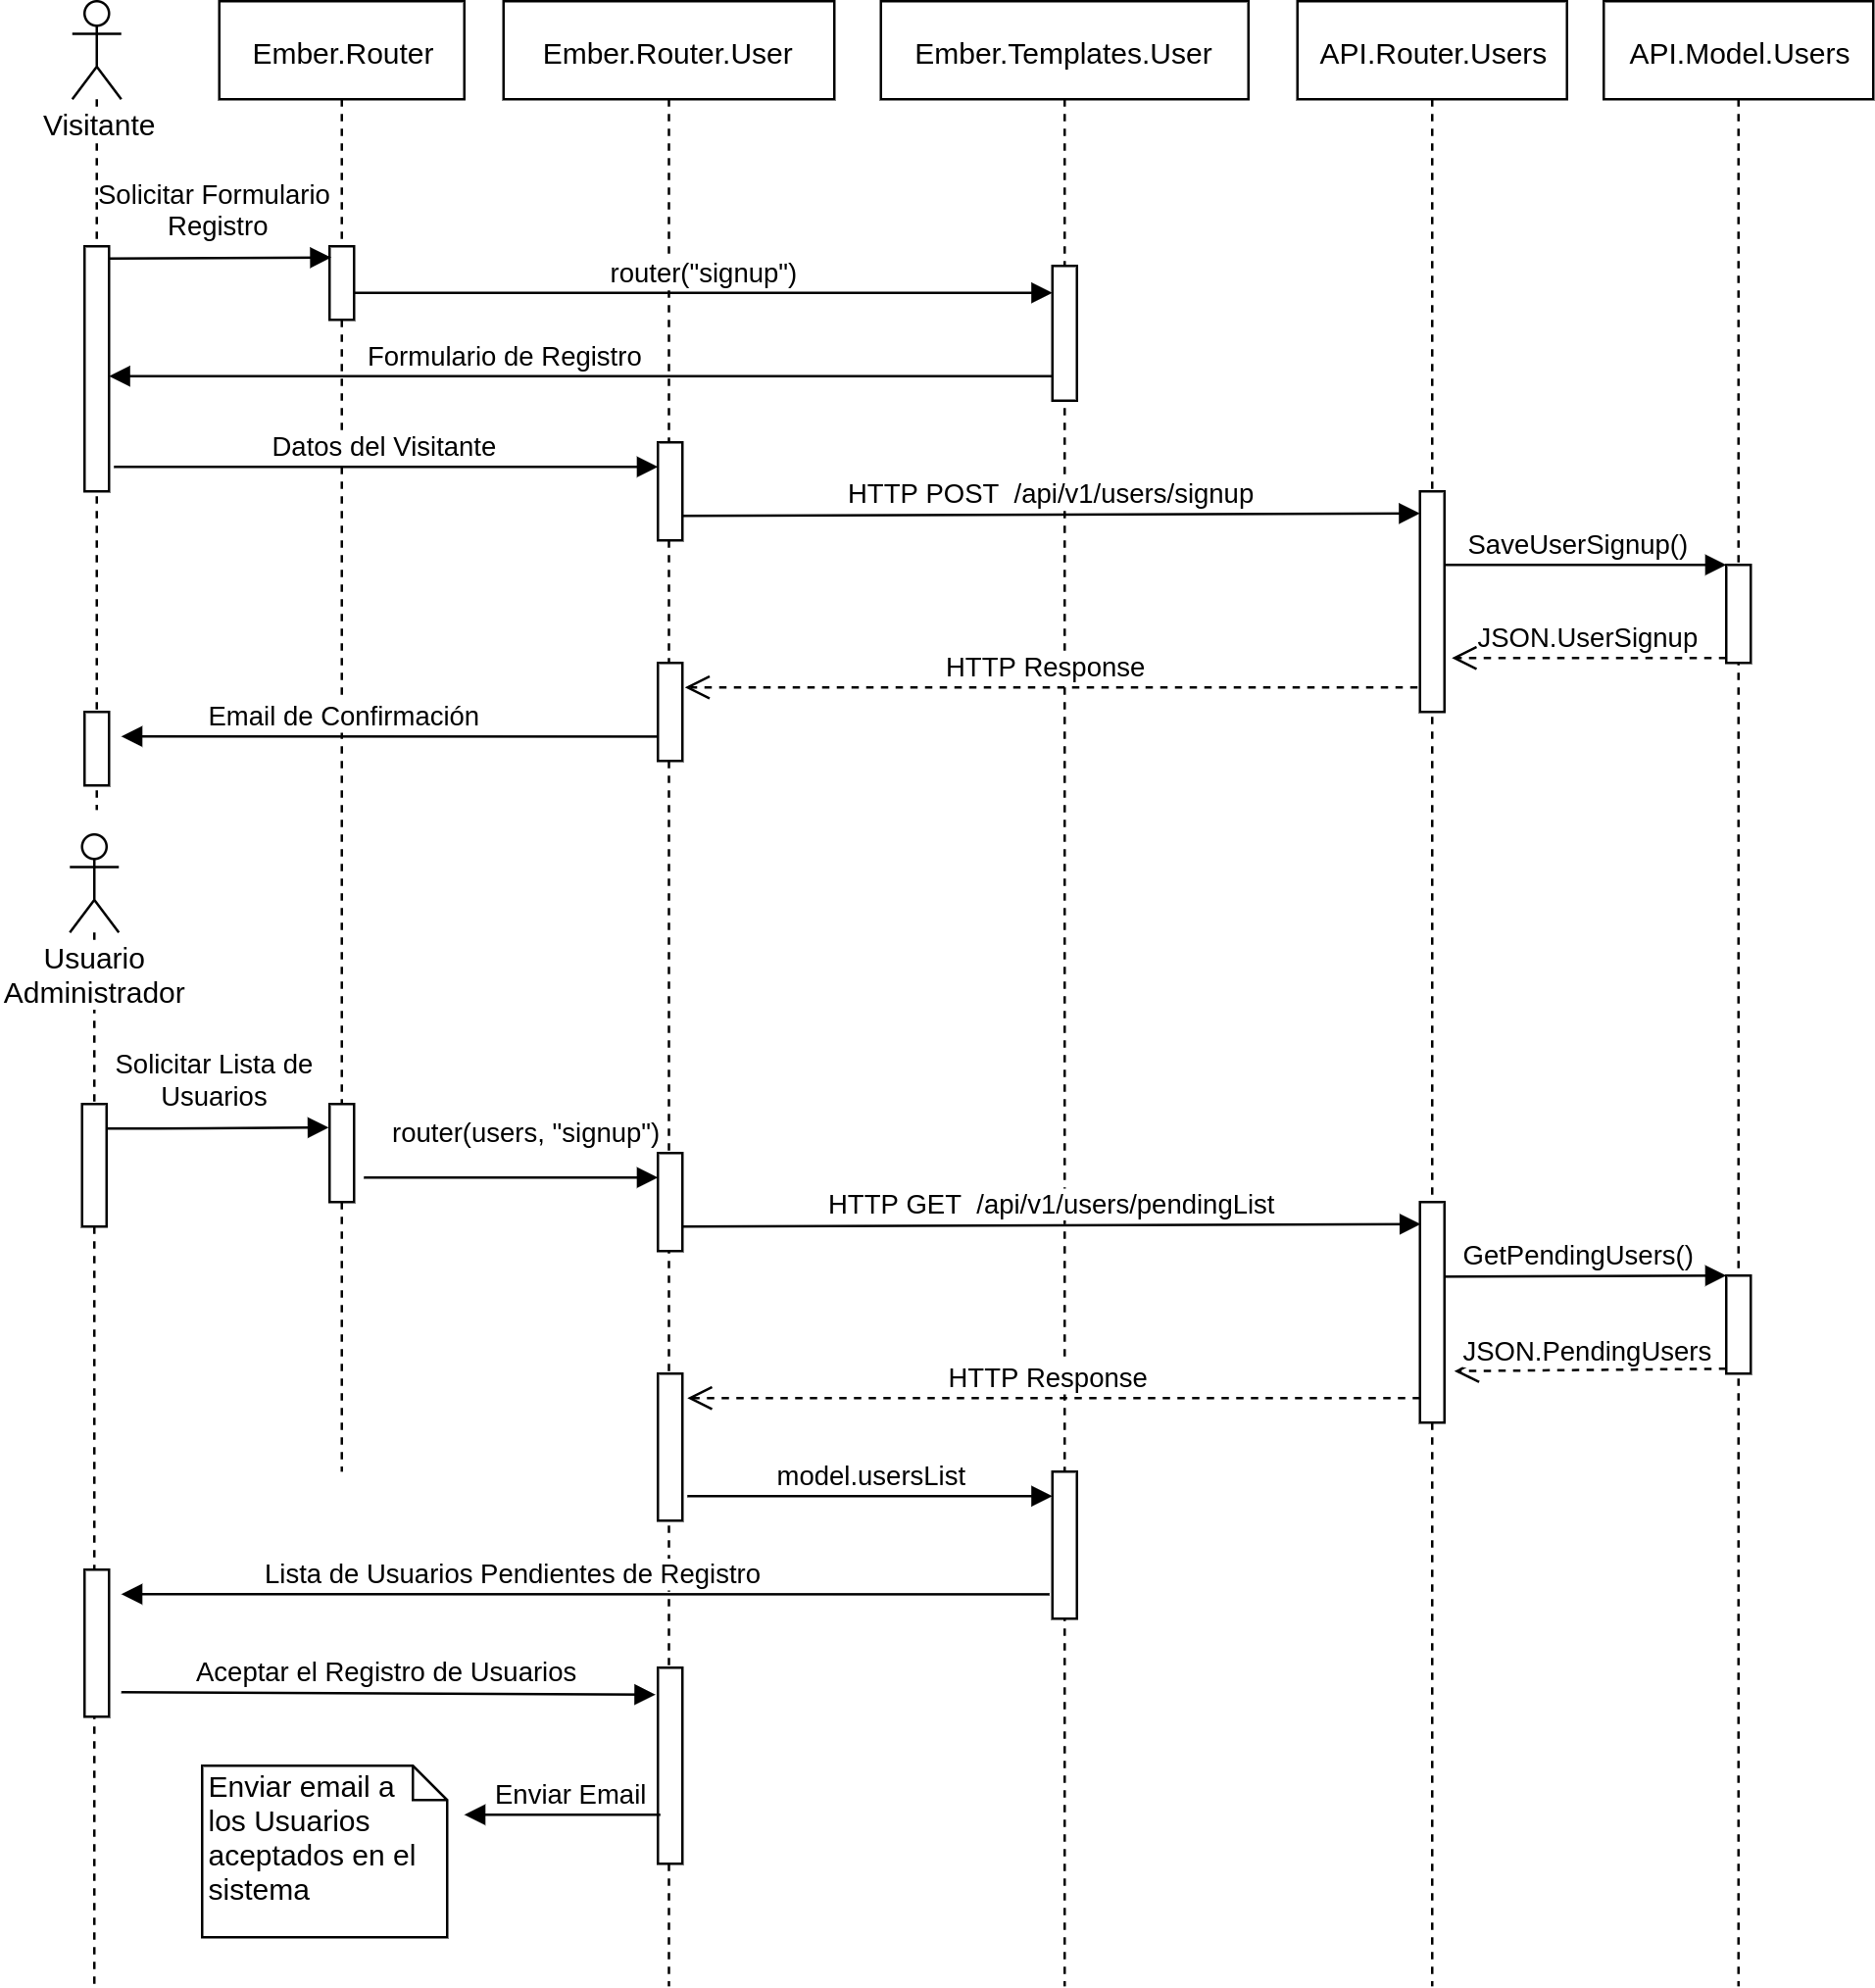
\includegraphics[width=0.9\textwidth]{diagramas/sequence_registrar_usuario}
  \end{center}
  \caption{Diagrama de Secuencia: Registrar Usuarios}
  \label{fig:sequence_registrar_usuario}
  \caption*{Fuente: Elaboración propia}
\end{figure}

En la figura \ref{fig:sequence_reporte}, se observa el diagrama de secuencia correspondiente a la obtención del reporte.

\begin{figure}[H]
  \begin{center}
    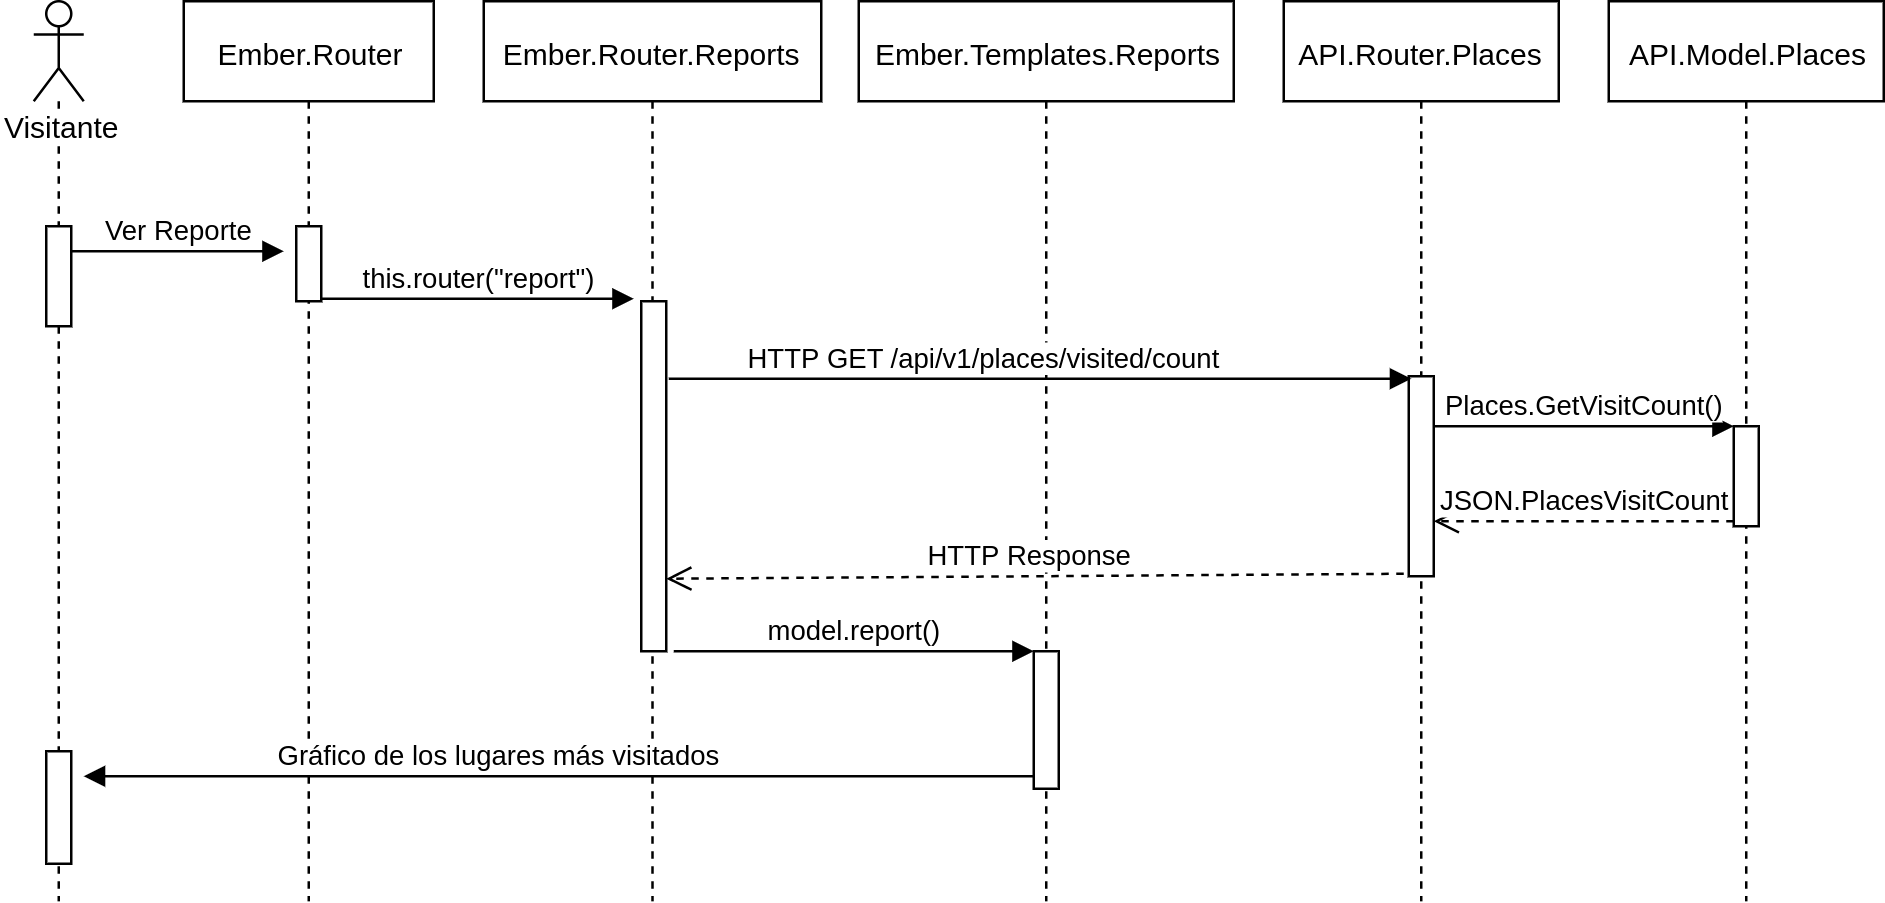
\includegraphics[width=0.9\textwidth]{diagramas/sequence_reporte}
  \end{center}
  \caption{Diagrama de Secuencia: Reporte}
  \label{fig:sequence_reporte}
  \caption*{Fuente: Elaboración propia}
\end{figure}


\newpage
\item \textbf{Diagrama de Clases:}

En la figura \ref{fig:clases_usuarios}, se observa el diagrama de clases correspondiente al registro de usuarios.

\begin{figure}[H]
\begin{center}
  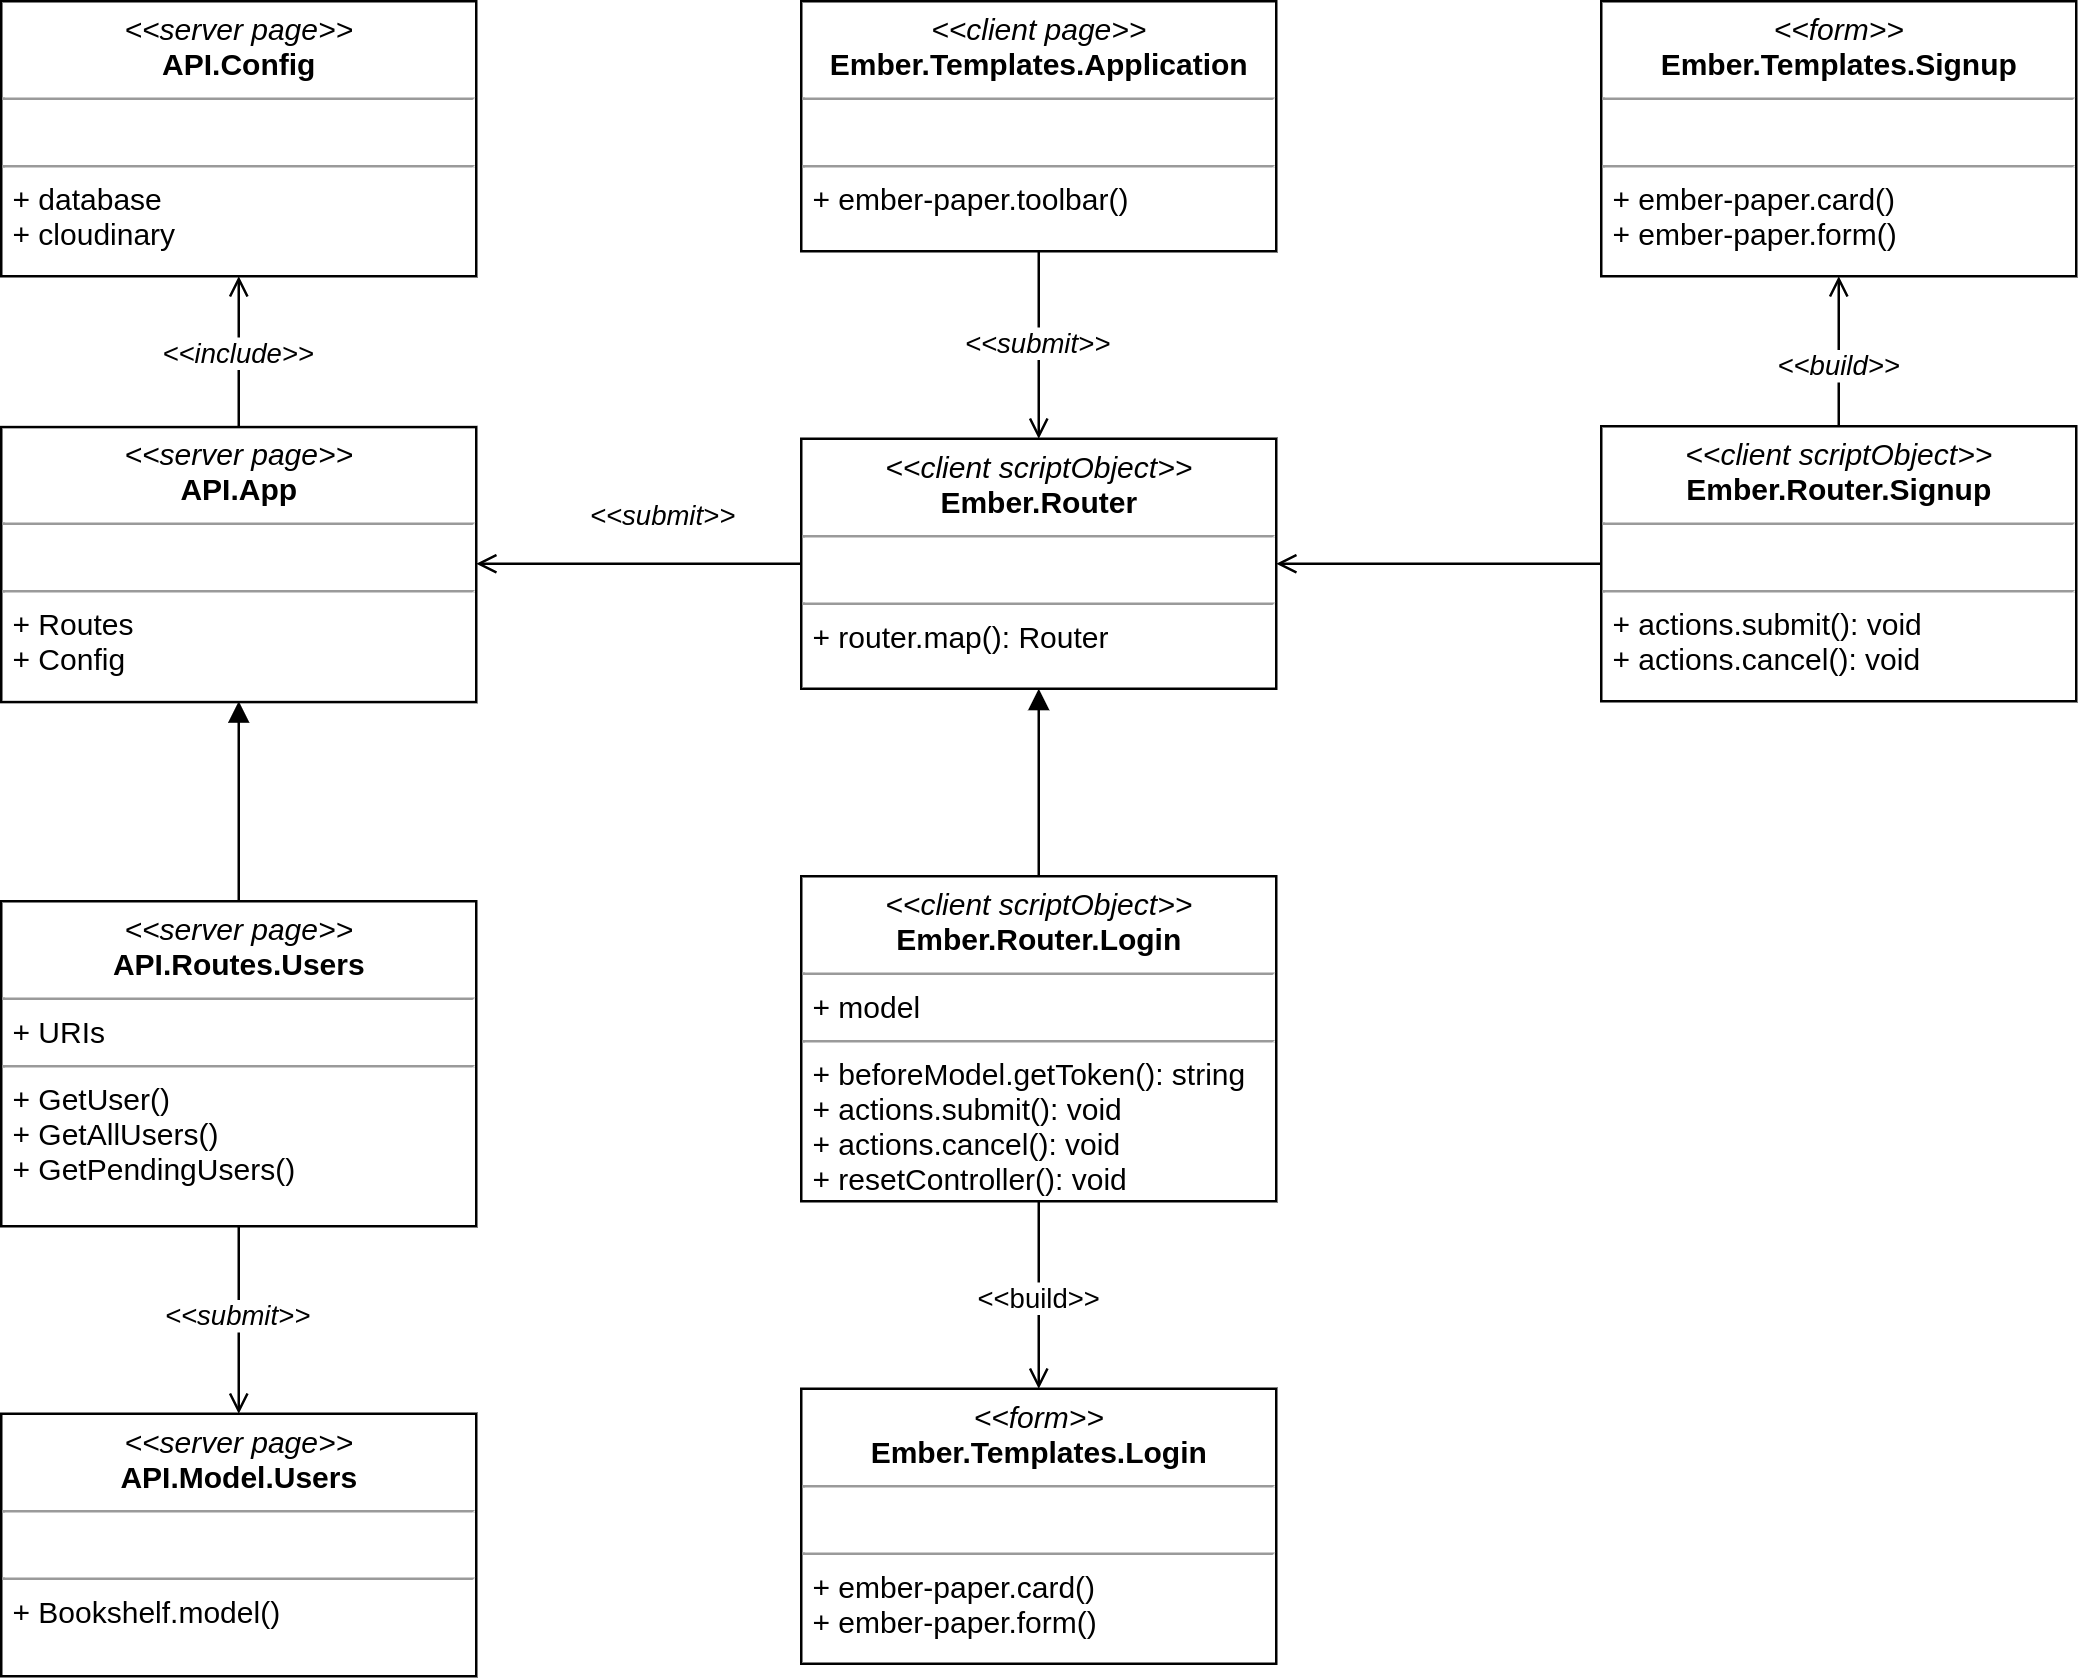
\includegraphics[width=0.9\textwidth]{diagramas/clases_usuarios}
\end{center}
\caption{Diagrama de Clases: Registro de Usuario}
\label{fig:clases_usuarios}
\caption*{Fuente: Elaboración propia}
\end{figure}


\end{itemize}
